% 依题目条件取 a=1：B=(0,0,0), A=(0,1,0), C=(1,0,0),
% D=(3,1,0), P=(0,1,1), E=(3/5,-1/5,0), H=(0,1/2,1/2)。
% 仿射投影基向量 (3,0)、(0.7,1.5)、(-0.4,2.5)；
% 保留平行、共线及中点关系，不以纸面角度表示空间直角。
\begin{center}
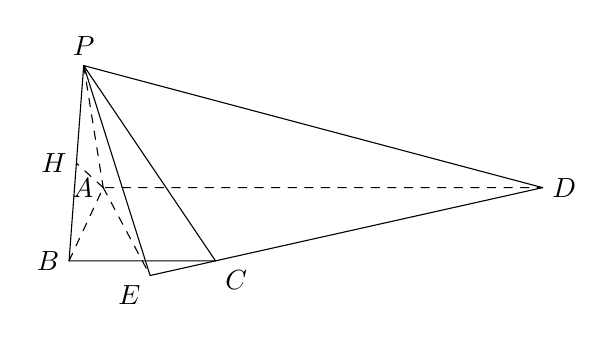
\begin{tikzpicture}[x=0.62cm,y=0.62cm,>=stealth,line cap=round,line join=round]
  \coordinate (B) at (0,0);
  \coordinate (A) at (0.7,1.5);
  \coordinate (C) at (3,0);
  \coordinate (D) at (9.7,1.5);
  \coordinate (P) at (0.3,4);
  \coordinate (E) at (1.66,-0.3);
  \coordinate (H) at (0.15,2);
  \draw (B)--(C)--(D);
  \draw[dashed] (B)--(A)--(D) (P)--(A);
  \draw (P)--(B) (P)--(C) (P)--(D);
  \draw[dashed] (A)--(E) (A)--(H);
  \draw (P)--(E) (E)--(C);
  \node[left] at (A) {$A$};
  \node[left] at (B) {$B$};
  \node[below right] at (C) {$C$};
  \node[right] at (D) {$D$};
  \node[above] at (P) {$P$};
  \node[below left] at (E) {$E$};
  \node[left] at (H) {$H$};
\end{tikzpicture}
\end{center}
